\chapter{\ifproject%
\ifenglish Project Structure and Methodology\else โครงสร้างและขั้นตอนการทำงาน\fi
\else%
\ifenglish Project Structure\else โครงสร้างของโครงงาน\fi
\fi
}

\makeatletter

% \renewcommand\section{\@startsection {section}{1}{\z@}%
%                                    {13.5ex \@plus -1ex \@minus -.2ex}%
%                                    {2.3ex \@plus.2ex}%
%                                    {\normalfont\large\bfseries}}

\makeatother
%\vspace{2ex}
% \titleformat{\section}{\normalfont\bfseries}{\thesection}{1em}{}
% \titlespacing*{\section}{0pt}{10ex}{0pt}

\section{หลักการและการออกแบบการทดลอง (Methodology \& Experimental Design)}


\begin{figure}[h!]
\centering
\resizebox{\textwidth}{!}{%
% ปรับสเกลเพื่อให้พอดีกับหน้ากระดาษหากจำเป็น
\begin{tikzpicture}[node distance=1.2cm and 1.5cm, auto, scale=0.8, transform shape]

    % --- วางตำแหน่งบล็อก (Nodes) ---
    
    % แถวบนสุด (Main Flow)
    \node (prep) [process] {Data Preparation};
    \node (train) [process, right=of prep] {Train};
    \node (post) [greyblock, right=of train] {Postprocess};
    \node (test) [process, right=of post] {Test};
    \node (eval) [process, right=of test] {Evaluation};
    
    % แถวที่สอง (Decision & Output)
    \node (decide) [decision, below=of eval, yshift=-0.5cm] {Can accuracy be\\improved by data?};
    \node (end) [endblock, below=of test, xshift=2.5cm, yshift=-0.5cm] {End};
    
    % แถวที่สาม (Refinement Path)
    \node (dataset) [datablock, below=of decide, yshift=-0.5cm] {Dataset};
    \node (pre) [greyblock, below left=of dataset, xshift=-0.5cm] {Preprocess};
    \node (add) [datablock, below right=of dataset, xshift=0.5cm] {Add dataset};
    
    % บล็อก List รายละเอียด (วางตำแหน่งสัมพัทธ์กับ Train และ Postprocess)
    \node (details) [listblock, below=of train, xshift=1.5cm, yshift=-0.8cm] {
        \textbullet\ Redo masks \\
        \textbullet\ Handling mirrored images \\
        \textbullet\ Anatomical correctness \\
        \hspace{0.3cm} checking \\
        \textbullet\ Object size distribution analysis \\
        \textbullet\ Tissue ratio analysis in \\
        \hspace{0.3cm} standard views
    };

    % --- ลากเส้นเชื่อมต่อ (Edges) ---
    
    % เส้นหลักแถวบน
    \draw [arrow] (prep) -- (train);
    \draw [arrow] (train) -- (post);
    \draw [arrow] (post) -- (test);
    \draw [arrow] (test) -- (eval);
    
    % เส้นจาก Evaluation ไปยังคำตัดสิน
    \draw [arrow] (eval) -- (decide);
    
    % เส้นคำตัดสิน (Yes/No)
    \draw [arrow] (decide) -- node[anchor=west] {Yes} (dataset);
    \draw [arrow] (decide.east) -| node[anchor=south, xshift=-1cm] {No} (end.north);
    
    % เส้นทางแยกจาก Dataset
    \draw [arrow] (dataset.south) -| (pre.north);
    \draw [arrow] (dataset.south) -| (add.north);
    
    % เส้นประ
    \draw [dashedline] (details.east) -- ++(0.3cm,0) |- (pre.north east);
    
    % --- เส้นย้อนกลับที่ซับซ้อน (Loop Backs) ---
    
    % เส้นจาก Preprocess กลับไป Postprocess
    % ลากลง -> ซ้าย -> ขึ้น -> เข้าบล็อก
    \draw [arrow] (pre.south) -- ++(0,-0.5cm) -- ++(0.5cm,0) |- (post.south);
    
    % เส้นย้อนกลับทั้งหมดไปยัง Data Preparation
    % ลากลง -> ซ้าย -> ขึ้น -> เข้าบล็อก
    % จุดเชื่อมใต้ Preprocess และ Add Dataset
    \coordinate (bottomloop) at ($(pre.south) + (0,-0.8cm)$);
    \draw [thick] (pre.south) -- ++(0,-0.8cm);
    \draw [thick] (add.south) -- ++(0,-0.8cm);
    
    % ลากเส้นยาวกลับไปหา Data Preparation
    \draw [arrow] (add.south) -- ++(0,-0.8cm) -- (prep.south |- bottomloop) -- (prep.south);
    
    % เส้นประจากรายละเอียดไปยังเส้นย้อนกลับหลัก
    \draw [dashedline] (details.west) -- ++(-0.2cm,0) |- (prep.south |- bottomloop);
    
    % ข้อความ "Refined dataset" (วางบนเส้น)
    \node [font=\sffamily\bfseries\small, anchor=east] at (prep.south |- details.west) {Refined dataset};

\end{tikzpicture}
}
\caption{แผนผังขั้นตอนการพัฒนาแบบจำลองและการปรับปรุงชุดข้อมูลโดยละเอียด}
\label{fig:detailed_workflow}
\end{figure}





\section{Model Selection}

ในการศึกษาครั้งนี้ได้ทำการคัดเลือกโมเดล (Model Selection) ซึ่งได้เลือก โมเดลจาก github qubvel/segmentation\_models \cite{Yakubovskiy:2019} โดยเลือก encoder และ decoder มาอย่างละ 5 อัน รวมทั้งสิน 25 โมเดล เพื่อนำมาทดสอบประสิทธิภาพกับชุดข้อมูล (Dataset) ของเรา โดยมีผลการทดสอบของโมเดลทั้งหมดที่ใช้ในการทดลองดังตารางที่ \ref{tab:all_models} ซึ่งแสดงค่า F1-Score, IoU และ Inference Time (วินาทีต่อรูปภาพ)

\begin{table}[hbt!]
\centering
\caption{ผลการทดสอบของโมเดลทั้ง 25 โมเดล}
\label{tab:all_models}
\begin{tabular}{|c|l|c|c|c|}
\hline
\textbf{ลำดับ} & \textbf{ชื่อโมเดล (Model)} & \textbf{F1-Score} & \textbf{IoU} & \textbf{Inference Time (s)} \\
\hline
1 & Linknet-resnet101 & 0.8263 & 0.7138 & 0.6688 \\
2 & UPerNet-resnet101 & 0.8240 & 0.7103 & 0.9418 \\
3 & Linknet-resnet50 & 0.8194 & 0.7055 & 0.4635 \\
4 & Unet-efficient-b7 & 0.8163 & 0.7010 & 0.9906 \\
5 & DeepLabV3-resnet101 & 0.8134 & 0.6955 & 0.6985 \\
6 & Unet-efficient-b3 & 0.8130 & 0.6964 & 0.4019 \\
7 & Unet-resnet & 0.8121 & 0.6951 & 0.7081 \\
8 & DeepLabV3-resnet50 & 0.8099 & 0.6916 & 0.4979 \\
9 & FPN-efficient-b3 & 0.8090 & 0.6904 & 0.3692 \\
10 & UPerNet-efficient-b7 & 0.8084 & 0.6908 & 1.2527 \\
11 & UPerNet-resnet50 & 0.8073 & 0.6875 & 0.8029 \\
12 & FPN-resnet101 & 0.8057 & 0.6854 & 0.6163 \\
13 & DeepLabV3-mobilenet\_v2 & 0.8050 & 0.6837 & 0.1927 \\
14 & DeepLabV3-efficientnet-b7 & 0.8036 & 0.6833 & 1.3603 \\
15 & Unet-resnet50 & 0.8022 & 0.6844 & 0.5174 \\
16 & UPerNet-efficient-b3 & 0.8000 & 0.6791 & 0.6915 \\
17 & Unet-mobilenet\_v2 & 0.7954 & 0.6729 & 0.2356 \\
18 & DeepLabV3-efficientnet-b3 & 0.7945 & 0.6728 & 0.3783 \\
19 & FPN-efficient-b7 & 0.7927 & 0.6699 & 1.0059 \\
20 & Linknet-efficient-b3 & 0.7920 & 0.6923 & 0.3146 \\
21 & UPerNet-mobilenet\_v2 & 0.7908 & 0.6658 & 0.5157 \\
22 & FPN-mobilenet\_v2 & 0.7863 & 0.6592 & 0.2116 \\
23 & FPN-resnet50 & 0.7830 & 0.6543 & 0.4201 \\
24 & Linknet-efficient-b7 & 0.7755 & 0.6586 & 0.9310 \\
25 & Linknet-mobilenet\_v2 & 0.7583 & 0.6739 & 0.1310 \\
\hline
\multicolumn{2}{|c|}{\textbf{ค่าเฉลี่ย (Average)}} & \textbf{0.8018} & \textbf{0.6845} & \textbf{0.6127} \\
\hline
\end{tabular}
\end{table}

จากผลการทดสอบในตารางที่ \ref{tab:all_models} ในตอนแรกผู้วิจัยได้พิจารณาเลือกใช้โมเดล \textbf{Linknet-resnet101} เนื่องจากมีค่า F1-Score สูงที่สุด (0.8263) อย่างไรก็ตาม เมื่อพิจารณาผลลัพธ์ภาพกราฟิกจากการจำแนกจริง (Visual Inspection) พบว่าบริเวณขอบของวัตถุมีลักษณะแตกและไม่เรียบเนียน ซึ่งอาจส่งผลกระทบต่อความแม่นยำในการนำไปใช้งานจริง ดังนั้น ผู้วิจัยจึงได้เพิ่มตัวชี้วัด \textbf{Hausdorff Distance} เข้ามาเพื่อใช้ในการประเมินความคลาดเคลื่อนของขอบภาพอย่างละเอียดมากยิ่งขึ้น (โดยที่ค่า Hausdorff Distance ยิ่งต่ำยิ่งบ่งบอกถึงขอบที่แม่นยำและแนบเนียนมากขึ้น)

ผลการทำการทดสอบที่นำค่า Hausdorff Distance มาร่วมพิจารณาสำหรับทั้ง 25 โมเดล แสดงไว้ดังตารางที่ \ref{tab:all_models_hausdorff}

\begin{table}[hbt!]
\centering
\caption{ผลการทดสอบของโมเดลทั้ง 25 โมเดล โดยเพิ่มตัวชี้วัด Hausdorff Distance}
\label{tab:all_models_hausdorff}
\begin{tabular}{|c|l|c|c|c|c|}
\hline
\textbf{ลำดับ} & \textbf{ชื่อโมเดล (Model)} & \textbf{F1-Score} & \textbf{IoU} & \textbf{Hausdorff} & \textbf{Inference Time (s)} \\
\hline
1 & Linknet-resnet101 & 0.8263 & 0.7138 & 78.2667 & 0.6688 \\
2 & UPerNet-resnet101 & 0.8240 & 0.7103 & 52.3718 & 0.9418 \\
3 & Linknet-resnet50 & 0.8194 & 0.7055 & 74.4905 & 0.4635 \\
4 & Unet-efficient-b7 & 0.8163 & 0.7010 & 77.1968 & 0.9906 \\
5 & DeepLabV3-resnet101 & 0.8134 & 0.6955 & 55.7222 & 0.6985 \\
6 & Unet-efficient-b3 & 0.8130 & 0.6964 & 74.7506 & 0.4019 \\
7 & Unet-resnet & 0.8121 & 0.6951 & 77.0389 & 0.7081 \\
8 & DeepLabV3-resnet50 & 0.8099 & 0.6916 & 56.9831 & 0.4979 \\
9 & FPN-efficient-b3 & 0.8090 & 0.6904 & 60.5217 & 0.3692 \\
10 & UPerNet-efficient-b7 & 0.8084 & 0.6908 & 57.7180 & 1.2527 \\
11 & UPerNet-resnet50 & 0.8073 & 0.6875 & 59.2978 & 0.8029 \\
12 & FPN-resnet101 & 0.8057 & 0.6854 & 55.6652 & 0.6163 \\
13 & DeepLabV3-mobilenet\_v2 & 0.8050 & 0.6837 & 58.6067 & 0.1927 \\
14 & DeepLabV3-efficientnet-b7 & 0.8036 & 0.6833 & 55.8317 & 1.3603 \\
15 & Unet-resnet50 & 0.8022 & 0.6844 & 74.7560 & 0.5174 \\
16 & UPerNet-efficient-b3 & 0.8000 & 0.6791 & 62.0261 & 0.6915 \\
17 & Unet-mobilenet\_v2 & 0.7954 & 0.6729 & 74.3620 & 0.2356 \\
18 & DeepLabV3-efficientnet-b3 & 0.7945 & 0.6728 & 57.6671 & 0.3783 \\
19 & FPN-efficient-b7 & 0.7927 & 0.6699 & 66.2021 & 1.0059 \\
20 & Linknet-efficient-b3 & 0.7920 & 0.6923 & 198.9889 & 0.3146 \\
21 & UPerNet-mobilenet\_v2 & 0.7908 & 0.6658 & 63.5663 & 0.5157 \\
22 & FPN-mobilenet\_v2 & 0.7863 & 0.6592 & 69.1811 & 0.2116 \\
23 & FPN-resnet50 & 0.7830 & 0.6543 & 65.4966 & 0.4201 \\
24 & Linknet-efficient-b7 & 0.7755 & 0.6586 & 141.6082 & 0.9310 \\
25 & Linknet-mobilenet\_v2 & 0.7583 & 0.6739 & 230.5526 & 0.1310 \\
\hline
\multicolumn{2}{|c|}{\textbf{ค่าเฉลี่ย (Average)}} & \textbf{0.8018} & \textbf{0.6845} & \textbf{79.9547} & \textbf{0.6127} \\
\hline
\end{tabular}
\end{table}

จากตารางที่ \ref{tab:all_models_hausdorff} ภายหลังจากที่ได้เพิ่มตัวชี้วัด Hausdorff Distance เข้ามาพิจารณาร่วมด้วย พบว่าโมเดลสถาปัตยกรรมกลุ่ม Linknet ทุกตัวมีค่า Hausdorff Distance ที่ค่อนข้างสูงมากอย่างเห็นได้ชัด และโมเดลในกลุ่ม Unet ก็มีค่าตัวชี้วัดนี้ในระดับที่สูงพอๆ กัน ซึ่งค่า Hausdorff Distance ที่สูงนั้นบ่งบอกถึงผลลัพธ์ของขอบภาพที่ไม่แนบเนียนและมีความคลาดเคลื่อนสูง ฉะนั้น เราจึงได้คัดกรองโดยสร้างตารางใหม่ที่จะทำการลบโมเดลในกลุ่ม Linknet และ Unet ออกทั้งหมด เพื่อให้เหลือเฉพาะกลุ่มโมเดลที่ให้ความสำคัญกับรายละเอียดของขอบเขตได้ดียิ่งขึ้น

\begin{table}[hbt!]
\centering
\caption{ผลการทดสอบของโมเดลหลังจากตัดกลุ่ม Linknet และ Unet ออก}
\label{tab:filtered_models_no_linknet_unet}
\begin{tabular}{|c|l|c|c|c|c|}
\hline
\textbf{ลำดับ} & \textbf{ชื่อโมเดล (Model)} & \textbf{F1-Score} & \textbf{IoU} & \textbf{Hausdorff} & \textbf{Inference Time (s)} \\
\hline
2 & UPerNet-resnet101 & 0.8240 & 0.7103 & 52.3718 & 0.9418 \\
5 & DeepLabV3-resnet101 & 0.8134 & 0.6955 & 55.7222 & 0.6985 \\
8 & DeepLabV3-resnet50 & 0.8099 & 0.6916 & 56.9831 & 0.4979 \\
9 & FPN-efficient-b3 & 0.8090 & 0.6904 & 60.5217 & 0.3692 \\
10 & UPerNet-efficient-b7 & 0.8084 & 0.6908 & 57.7180 & 1.2527 \\
11 & UPerNet-resnet50 & 0.8073 & 0.6875 & 59.2978 & 0.8029 \\
12 & FPN-resnet101 & 0.8057 & 0.6854 & 55.6652 & 0.6163 \\
13 & DeepLabV3-mobilenet\_v2 & 0.8050 & 0.6837 & 58.6067 & 0.1927 \\
14 & DeepLabV3-efficientnet-b7 & 0.8036 & 0.6833 & 55.8317 & 1.3603 \\
16 & UPerNet-efficient-b3 & 0.8000 & 0.6791 & 62.0261 & 0.6915 \\
18 & DeepLabV3-efficientnet-b3 & 0.7945 & 0.6728 & 57.6671 & 0.3783 \\
19 & FPN-efficient-b7 & 0.7927 & 0.6699 & 66.2021 & 1.0059 \\
21 & UPerNet-mobilenet\_v2 & 0.7908 & 0.6658 & 63.5663 & 0.5157 \\
22 & FPN-mobilenet\_v2 & 0.7863 & 0.6592 & 69.1811 & 0.2116 \\
23 & FPN-resnet50 & 0.7830 & 0.6543 & 65.4966 & 0.4201 \\
\hline
\multicolumn{2}{|c|}{\textbf{ค่าเฉลี่ยใหม่ (New Average)}} & \textbf{0.8022} & \textbf{0.6813} & \textbf{59.7905} & \textbf{0.6637} \\
\hline
\end{tabular}
\end{table}

จากนั้น เพื่อที่จะคัดเลือกโมเดลที่มีประสิทธิภาพสูงสุดและมีความเหมาะสมที่สุดสำหรับการนำไปใช้งาน ผู้วิจัยได้ตั้งเกณฑ์การคัดกรองขั้นสุดท้ายอย่างเข้มงวด โดยอ้างอิงจากค่าเฉลี่ยใหม่ในตารางที่ \ref{tab:filtered_models_no_linknet_unet} ซึ่งหากมีโมเดลใดที่มีตัวชี้วัดแม้เพียงตัวเดียวที่ให้ผลลัพธ์ด้อยกว่าค่าเฉลี่ยนี้ (กล่าวคือ มีค่า F1-Score ต่ำกว่า 0.8022 หรือ IoU ต่ำกว่า 0.6813 หรือมีค่า Hausdorff Distance สูงกว่า 59.7905 หรือ Inference Time สูงกว่า 0.6637 วินาที) โมเดลนั้นจะถูกคัดออกจากการพิจารณาทันที

ผลลัพธ์จากการคัดกรองพบว่า มีโมเดลที่ผ่านเกณฑ์ดังกล่าวและทำคะแนนได้ดีกว่าค่าเฉลี่ยในครบทุกตัวชี้วัดจำนวนทั้งสิ้น 3 โมเดล ซึ่งแสดงรายละเอียดเป็นตารางสรุปผลสุดท้ายดังตารางที่ \ref{tab:final_filtered_models}

\begin{table}[hbt!]
\centering
\caption{ผลการทดสอบของโมเดลที่ผ่านเกณฑ์สุดท้าย (ทุกตัวชี้วัดดีกว่าหรือเท่ากับค่าเฉลี่ยใหม่)}
\label{tab:final_filtered_models}
\begin{tabular}{|c|l|c|c|c|c|}
\hline
\textbf{ลำดับ} & \textbf{ชื่อโมเดล (Model)} & \textbf{F1-Score} & \textbf{IoU} & \textbf{Hausdorff} & \textbf{Inference Time (s)} \\
\hline
8 & DeepLabV3-resnet50 & 0.8099 & 0.6916 & 56.9831 & 0.4979 \\
12 & FPN-resnet101 & 0.8057 & 0.6854 & 55.6652 & 0.6163 \\
13 & DeepLabV3-mobilenet\_v2 & 0.8050 & 0.6837 & 58.6067 & 0.1927 \\
\hline
\multicolumn{2}{|c|}{\textbf{ค่าเฉลี่ยสุดท้าย (Final Average)}} & \textbf{0.8069} & \textbf{0.6869} & \textbf{57.0850} & \textbf{0.4356} \\
\hline
\end{tabular}
\end{table}

อย่างไรก็ตาม เนื่องจากตัวชี้วัด IoU และ F1-Score มีลักษณะการประเมินความแม่นยำและทิศทางของผลลัพธ์ที่คล้ายคลึงกัน (ประเมินความทับซ้อนของพื้นที่การทำนายและเฉลย) ผู้วิจัยจึงได้พิจารณาตัดการพิจารณาด้าน IoU ออกในขั้นตอนสุดท้ายเพื่อลดความซ้ำซ้อน จากนั้นจึงนำตัวชี้วัดที่เหลือทั้ง 3 ตัว ได้แก่ F1-Score, Hausdorff Distance และ Inference Time มาทำการจัดอันดับ (Ranking) แบบ 1 ถึง 3 (โดยอันดับ 1 คืออันดับที่ดีที่สุด) สำหรับทั้ง 3 โมเดลสุดท้าย เพื่อค้นหาโมเดลที่มีความสมดุลและมีประสิทธิภาพโดยรวมสูงที่สุด ดังผลลัพธ์การจัดอันดับที่แสดงในตารางที่ \ref{tab:model_ranking}

\begin{table}[hbt!]
\centering
\caption{ผลการจัดอันดับโมเดล (Ranking) จาก 3 ตัวชี้วัดที่เหลือ}
\label{tab:model_ranking}
\begin{tabularx}{\textwidth}{|c|>{\raggedright\arraybackslash}X|c|c|c|c|} % ใช้ X เพื่อให้คอลัมน์ยืดหยุ่น
\hline
\textbf{ลำดับ} & \textbf{ชื่อโมเดล (Model)} & \textbf{Rank (F1)} & \textbf{Rank (HD)} & \textbf{Rank (Inf)} & \textbf{คะแนนรวม} \\
\hline
8 & DeepLabV3-resnet50 & 1 & 2 & 2 & \textbf{5} \\
12 & FPN-resnet101 & 2 & 1 & 3 & 6 \\
13 & DeepLabV3-mobilenet\_v2 & 3 & 3 & 1 & 7 \\
\hline
\end{tabularx}
\end{table}

จากตารางที่ \ref{tab:model_ranking} จะพบว่าเมื่อนำอันดับจากทั้ง 3 ตัวชี้วัดมารวมกัน โมเดล \textbf{DeepLabV3-resnet50} มีผลรวมของคะแนนอันดับที่น้อยที่สุด (5 คะแนน) ซึ่งแสดงให้เห็นอย่างชัดเจนถึงความสมดุลที่ยอดเยี่ยมระหว่างความแม่นยำที่สูงที่สุด (อันดับ 1 ในด้าน F1-Score) ความทนทานและความแม่นยำด้านขอบเขตของภาพ (อันดับ 2 ด้าน Hausdorff) รวมถึงความรวดเร็วในการประมวลผล (อันดับ 2 ด้าน Inference Time) ด้วยเหตุนี้ในงานวิจัยนี้ จึงได้ตัดสินใจคัดเลือกโมเดล \textbf{DeepLabV3-resnet50} เพื่อนำไปใช้งานและพัฒนาจริงในขั้นตอนถัดไป

\section{การฝึกสอนแบบจำลอง (Train)}

ในการฝึกสอนแบบจำลอง (Train) ได้มีการกำหนดองค์ประกอบต่างๆ รวมถึงสัดส่วนข้อมูล ได้แก่ ชุดข้อมูลสำหรับฝึกสอน (Train) 80\%, ชุดข้อมูลสำหรับตรวจสอบความถูกต้อง (Validation) 10\% และชุดข้อมูลสำหรับทดสอบ (Test) 10\% 

สำหรับการตั้งค่าสำหรับการฝึกสอนตัวแบบ (Setup) และเทคนิคการเพิ่มความหลากหลายของข้อมูล (Data Augmentation) ได้มีการสรุปรายละเอียดไว้ดังตารางที่ \ref{tab:train_setup} และ \ref{tab:data_augmentation} ตามลำดับ

\begin{table}[hbt!]
\centering
\caption{การตั้งค่าพารามิเตอร์สำหรับการฝึกสอน (Hyperparameters Setup)}
\label{tab:train_setup}
\begin{tabular}{|l|l|}
\hline
\textbf{รายการพารามิเตอร์} & \textbf{รายละเอียด} \\
\hline
ขนาดภาพ (Image Size) & $512 \times 512$ พิกเซล \\
Optimizer & Adam \\
Learning Rate (เริ่มต้น) & $1 \times 10^{-4}$ \\
Batch Size & 16 \\
จำนวนรอบ (Epochs) & 100 \\
การหยุดก่อนกำหนด (Early Stopping) & 25 Epochs \\
การปรับลด Learning Rate & ลดครึ่งหนึ่งเมื่อ Val Loss นิ่ง 8 Epochs (ต่ำสุด $1 \times 10^{-7}$) \\
\hline
\end{tabular}
\end{table}

\begin{table}[hbt!]
\centering
\caption{การเพิ่มปริมาณและปรับแต่งข้อมูล (Data Augmentation)}
\label{tab:data_augmentation}
\begin{tabular}{|l|l|}
\hline
\textbf{เทคนิคที่ใช้งาน} & \textbf{รายละเอียด} \\
\hline
การพลิกภาพ (Horizontal Flip) & พลิกแนวนอนแบบสุ่ม \\
การหมุนภาพ (Rotation) & $-45^{\circ}$ ถึง $45^{\circ}$ \\
การเลื่อนภาพ (Translate) & $(0.1, 0.1)$ \\
การปรับอัตราส่วน (Scale) & $0.9$ ถึง $1.1$ \\
การปรับแต่งสี (Color Jitter) & ปรับความสว่าง, ความเปรียบต่าง, ความอิ่มตัว \\
การเบลอภาพ (Gaussian Blur) & เบลอเฉพาะบางส่วนของภาพ \\
\hline
\end{tabular}
\end{table}

\textbf{เหตุผลในการเลือกใช้ฟังก์ชันสูญเสีย (Loss Function):}
ในการฝึกสอนโมเดล มีการใช้งาน \textbf{Dice Loss} ร่วมกับ \textbf{Cross-Entropy Loss} สาเหตุหลักมาจากการที่ Cross-Entropy Loss เป็นฟังก์ชันมาตรฐานที่ช่วยประเมินและลดทอนความคลาดเคลื่อนในการพยากรณ์พิกเซล ทำให้เสถียรภาพของการแยกแยะคลาสโดยรวมทำงานได้นิ่งและเป็นธรรมชาติ ในขณะเดียวกัน ภาพในการแบ่งส่วนรอยโรคส่วนใหญ่มักประสบปัญหาความไม่สมดุลของคลาส (Class Imbalance) ระหว่างพื้นที่ส่วนที่เป็นรอยโรคกับพื้นที่ส่วนที่เป็นพื้นหลัง (Background) ซึ่งมีขนาดใหญ่กว่ามาก ดังนั้น การใช้ฟังก์ชัน Dice Loss ที่มุ่งเน้นไปที่ค่าความทับซ้อน (Intersection over Union) ร่วมด้วย จึงเป็นการช่วยบังคับให้โมเดลหันมาให้ความสำคัญกับคลาสที่เป็นรอยโรคที่มีขนาดเล็กกว่าอย่างมีประสิทธิภาพมากยิ่งขึ้น ส่งผลให้ความสมบูรณ์และพิกัดความแม่นยำของการจำแนกพื้นที่ (Segmentation accuracy) มีประสิทธิภาพสูงสุด

\section{การทดสอบและประเมินผลสมรรถนะ (Test \& Evaluation)}

ภายหลังจากขั้นตอนการฝึกสอนตัวแบบ การทดสอบและประเมินผลสมรรถนะ (Test \& Evaluation) นับเป็นกระบวนการที่มีความสำคัญเพื่อประเมินขีดความสามารถที่แท้จริงของโมเดลสำหรับการนำไปใช้งาน โดยใช้ข้อมูลในส่วนของชุดทดสอบ (Test Set) ซึ่งเป็นรูปภาพที่ตัวแบบไม่เคยเห็นจากการฝีกสอนมาก่อนเลย (Unseen Data) ทำให้ผู้วิจัยสามารถสังเกตพัฒนาการและการเรียนรู้ประยุกต์ใช้ลักษณะเด่นของโมเดลต่อข้อมูลในสถานการณ์ที่เป็นรูปภาพใหม่ได้อย่างแม่นยำ

สำหรับการประเมินประสิทธิภาพของการแบ่งส่วน (Segmentation Evaluation) ในโปรเจกต์นี้ ตัวชี้วัดที่ถูกนำมาพิจารณาประกอบไปด้วย 5 ค่าหลัก ดังต่อไปนี้:
\begin{itemize}
    \item \textbf{Precision:} มาตรวัดความถูกต้องของการทำนาย ว่าจากทุกพิกเซลที่โมเดลระบุและตั้งความน่าจะเป็นว่าเป็นเนื้อเยื่อเป้าหมายหรือรอยโรค มีกี่พิกเซลที่เป็นความจริง
    \item \textbf{Recall:} สะท้อนให้เห็นว่า จากพื้นที่ที่เป็นรอยโรคทั้งหมดที่มีในภาพกราวด์ทรูธ (Ground Truth) โมเดลสามารถตรวจจับและทำนายครอบคลุมมากน้อยเพียงใด ช่วยชี้วัดถึงเนื้อเยื่อที่เป็นรอยโรคที่อาจบังเอิญถูกพลาดนำไป
    \item \textbf{F1-Score:} เป็นค่าเฉลี่ยฮาร์มอนิกของ Precision และ Recall เนื่องจากโดยทั่วไปตัวชี้วัดทั้งสองมักจะทำงานสวนทางกัน ค่า F1-Score จึงทำให้เราเห็นสมดุลและความน่าเชื่อถือภายใต้ความซับซ้อนของข้อมูล
    \item \textbf{Intersection over Union (IoU):} ประเมินตัวเลขพิกัดความทับซ้อนเชิงพื้นที่ระหว่างสิ่งที่โมเดลทำนายได้กับพื้นที่จริง
    \item \textbf{Boundary F1 (BF-Score):} ตัวชี้วัดพิเศษที่คอยดูความแม่นยำของเส้นขอบ (Boundary) โดยพิจารณาระดับความสอดคล้องและความแคบของขอบเขตระหว่างสิ่งที่พยากรณ์ได้กับความเป็นจริง เพื่อดูว่าผลลัพธ์รอบนอกของรอยโรคแนบเนียนหรือไม่ อย่างที่ใช้คัดกรองตัวแบบในหัวข้อที่ \ref{tab:model_ranking} 
\end{itemize}

\textbf{เงื่อนไขสำคัญในการประเมินผล (Exclusion of Background):}
สิ่งที่เป็นข้อควรระวังอย่างยิ่งในการประเมินประสิทธิภาพการแบ่งส่วนภาพทางการแพทย์คือ สัดส่วนพิกเซลของรอยโรคแทบพ่ายแพ้ให้กับบริเวณพื้นที่ว่าง (Background) ซึ่งมักมีขนาดใหญ่มากกว่าอยู่เสมอ ถ้าหากนำไปคำนวณรวมด้วย จะส่งผลให้บรรดาค่าตัวชี้วัดถูกบิดเบือนและแสดงค่าสูงเกินความเป็นจริง (Overestimation) ดังนั้น ในการคำนวณวัดผลและหาค่าตัวชี้วัดความแม่นยำที่กล่าวมาทั้งหมดข้างต้น \textbf{ผู้วิจัยจะไม่นับรวมผลลัพธ์การทำนายในส่วนของพิกเซลบนคลาสที่เป็นพื้นหลัง (Background) มาคำนวณโดยเด็ดขาด} การเพิกเฉยต่อความถูกต้องส่วนพื้นที่โครงสร้างที่ไม่ใช่เป้าหมาย ทำให้ตัวชี้วัดสะท้อนผลลัพธ์ออกมาเป็นศักยภาพของโมเดลในการตรวจจัดโครงสร้างรอยโรคเป้าหมายล้วนๆ ซึ่งเป็นการประเมินที่มีความเข้มงวด ชัดเจน และสอดคล้องกับจุดประสงค์ของงานวิจัยอย่างเป็นรูปธรรม

\section{การทดลอง (Experiments)}

เพื่อประเมินประสิทธิภาพการทำงานของตัวแบบและศึกษาถึงผลกระทบจากการจัดเตรียมข้อมูล ทั้งก่อนเข้ากระบวนการฝึกสอน (Preprocessing) และภายหลังจากการได้รับผลลัพธ์ (Postprocessing) กระบวนการทดลองในงานวิจัยนี้จึงได้ถูกออกแบบและแบ่งออกเป็น 4 การทดลองหลักอย่างเป็นลำดับขั้น (Ablation/Progressive Study) ดังต่อไปนี้

นอกจากนี้ ในทุกการทดลอง ผู้วิจัยได้กำหนดแนวทางการฝึกสอนโดยใช้ชุดข้อมูลทั้งหมด (Full Dataset) เพื่อให้โมเดลสามารถเรียนรู้โครงสร้างทางกายภาพที่หลากหลายภายในช่องปากได้อย่างครบถ้วน แต่ในขั้นตอนการประเมินผล (Evaluation) จะมีการแยกชุดทดสอบออกเป็น 2 รูปแบบหลัก คือ การทดสอบกับภาพถ่ายช่องปากที่ไม่มีรอยโรค เพื่อประเมินความสามารถในการจำแนกพื้นที่ปกติโดยไม่เกิดความผิดพลาด (False Positive) และการทดสอบกับภาพถ่ายช่องปากที่มีรอยโรค เพื่อวัดความแม่นยำในการตรวจจับและแบ่งส่วนพื้นที่รอยโรคเป้าหมายที่แท้จริง

\subsection{การทดลองที่ 1: การฝึกสอนด้วยชุดข้อมูลดั้งเดิม (Baseline Training with Old Dataset)}
ในการทดลองแรก ผู้วิจัยได้ทำการฝึกสอนโมเดลโดยใช้ชุดข้อมูลดั้งเดิม (Old Dataset) จุดประสงค์หลักของการทดลองเบื้องต้นนี้คือการสร้างค่ามาตรฐานอ้างอิง (Baseline) สำหรับโครงข่ายประสาทเทียม เพื่อใช้ในการประเมินโครงสร้างหลักของสถาปัตยกรรมตัวแบบ ตลอดจนเพื่อเป็นเครื่องมือสังเกตปัญหาและข้อจำกัดต่างๆ ที่เกิดขึ้นจากความคลาดเคลื่อนของข้อมูลก่อนการปรับปรุงแก้ไข

\subsection{การทดลองที่ 2: การฝึกสอนด้วยชุดข้อมูลฉบับปรับปรุง (Training with New Dataset)}
ภายหลังจากการประเมินข้อบกพร่องของข้อมูลในเบื้องต้น ผู้วิจัยได้จัดทำและทำความสะอาดชุดข้อมูลใหม่ (New Dataset) ซึ่งผ่านกระบวนการตรวจสอบและปรับแก้คำตอบ (Ground Truth Labels) อย่างละเอียดถี่ถ้วนมากยิ่งขึ้น ในการทดลองที่สองนี้ โมเดลจะถูกฝึกสอนและทดสอบใหม่ทั้งหมดบนชุดข้อมูลฉบับปรับปรุง เพื่อพิสูจน์สมมติฐานสำคัญที่ว่า ข้อมูลคำสอนที่มีบรรทัดฐานและความถูกต้องสูงขึ้น จะประเมินและช่วยยกระดับความแม่นยำของผลลัพธ์ได้อย่างมีนัยสำคัญ

\subsection{การทดลองที่ 3: การประยุกต์ใช้เทคนิคการเตรียมข้อมูลภาพ (New Dataset + Preprocessing)}
เพื่อพยายามดึงศักยภาพการสกัดลักษณะเด่นของตัวแบบออกมาให้ได้สูงสุด ผู้วิจัยได้ดำเนินการต่อเนื่องจากการทดลองที่ 2 โดยการเพิ่มขั้นตอนการเตรียมข้อมูลภาพและการปรับสมดุล (Image Preprocessing) บางประการก่อนนำเข้าสู่กระบวนการฝึกสอน การทดลองนี้มุ่งตรวจสอบกลไกการเรียนรู้ ว่าการปรับปรุงคุณภาพและทำมาตรฐานเชิงภาพทัศน์ของรอยโรคจะสามารถช่วยให้ตัวแบบโฟกัสลักษณะรอยโรคและเพิ่มความทนทาน (Robustness) ในกระบวนการทำนายผลได้ดีขึ้นหรือไม่

\subsection{การทดลองที่ 4: การปรับจูนผลลัพธ์ด้วยกระบวนการตรวจแก้หลังการประมวล (New Dataset + Preprocessing + Postprocessing)}
สำหรับการทดลองขั้นสุดท้าย เป็นการประยุกต์ใช้ระเบียบวิธีจัดการภาพรวมแบบครบวงจร โดยต่อยอดจากการทดลองที่ 3 ด้วยการผนวกกระบวนการตรวจแก้หลังการประมวล (Postprocessing) หลังจากที่โมเดลได้ทำการประเมินผลการแบ่งส่วนพื้นที่ภาพเป็นที่เรียบร้อย กระบวนการนี้อาจครอบคลุมถึงการตรวจจับตัวพื้นที่ทำนายที่มีขนาดเล็กจนผิดปกติและดึงออก (Noise Removal) หรือการเติมเต็มช่องโหว่ (Hole Filling) การเปรียบเทียบผลลัพธ์ในการทดลองที่ 4 จะชี้วัดความสามารถในการสกัดกั้นผลบวกลวงหรือการฟื้นฟูข้อผิดพลาดของโมเดล เพื่อให้กราฟิกขอบเขตรอยโรคที่ถูกระบายสีทับมีความเรียบเนียนสมบูรณ์และนำไปประยุกต์ใช้ในบริบททางการแพทย์ได้เสมือนจริงมากที่สุด



\section{การจัดการข้อมูลและการเตรียมข้อมูล}
ผู้จัดทําได้รับชุดข้อมูลภาพถ่ายช่องปาก มาจากศูนย์ทันตสาธารณสุขระหว่างประเทศ กรมอนามัย กระทรวง
สาธารณสุข ซึ่งเป็นภาคีเครือข่ายวิจัยเดียวกันกับผู้จัดทํา ทั้งนี้ทันตแพทย์ ทันตบุคลากร และเจ้าหน้าที่ของ
กระทรวงสาธารณสุขภายใต้หน่วยงานดังกล่าวจะเป็นผู้เก็บรวบรวมข้อมูล และมีภารกิจในการลงพื้นที่ตาม
ชุมชนต่าง ๆ เพื่อตรวจคัดกรองหารอยโรคก่อนมะเร็งและรอยโรคมะเร็งช่องปาก ทางผู้จัดทําได้คัดเลือกภาพ
ที่ไม่ซํ้ากันมาจากชุดข้อมูลดังกล่าวเป็นจํานวน 1,692 ภาพ โดยแบ่งเป็นภาพที่มีรอยโรคก่อนมะเร็งและรอยโรคมะเร็งช่องปาก 1,259 ภาพ และภาพที่ไม่มีรอยโรค 433 ภาพ และแบ่งออกเป็น 9 มุมมองมาตรฐาน ได้แก่ มุมมองกระพุ้งแก้ม (Buccal mucosa view), มุมมองด้านหลังลิ้นและด้านข้างลิ้น (Dorsal and lateral tongue view), มุมมองพื้นปาก (Floor of mouth view), มุมมองเหงือก (Gingiva view), มุมมองเพดานปาก (Hard and Soft palate views), มุมมองริมฝีปาก (Lips view), มุมมองเหงือกด้านหลังฟันกรามล่าง (Retromolar pad view) และมุมมองลิ้นด้านล่าง (Ventral tongue view) โดยมีจำนวนภาพแบ่งตามมุมมองมาตรฐานและประเภทของรอยโรคดังแสดงในตารางที่ \ref{tab:oral_lesion_data}

\begin{table}[htbp]
    \centering
    \caption{ตารางแสดงจำนวนภาพแบ่งตามมุมมองมาตรฐานและประเภทของรอยโรค}
    \label{tab:oral_lesion_data}
    \begin{tabular}{|l|c|c|}
        \hline
        \textbf{มุมมองมาตรฐาน (Standard View)} & \textbf{ภาพไม่มีรอยโรค} & \textbf{ภาพที่มีรอยโรค} \\ \hline
        มุมมองกระพุ้งแก้ม (Buccal mucosa view) & 242 & 149 \\ \hline
        มุมมองด้านหลังลิ้นและด้านข้างลิ้น (Dorsal and lateral tongue view) & 195 & 73 \\ \hline
        มุมมองพื้นปาก (Floor of mouth view) & 79 & 43 \\ \hline
        มุมมองเหงือก (Gingiva view) & 150 & 80 \\ \hline
        มุมมองเพดานปาก (Hard and Soft palate views) & 78 & 18 \\ \hline
        มุมมองริมฝีปาก (Lips view) & 243 & 23 \\ \hline
        มุมมองเหงือกด้านหลังฟันกรามล่าง (Retromolar pad view) & 158 & 34 \\ \hline
        มุมมองลิ้นด้านล่าง (Ventral tongue view) & 114 & 13 \\ \hline
        \textbf{รวมทั้งหมด} & \textbf{1259} & \textbf{433} \\ \hline
    \end{tabular}
\end{table}

จากนั้นทำการสร้างผลเฉลย (Ground truth) ด้วยเว็บแอปพลิเคชัน Labelbox ~\cite{labelbox} โดยให้ทันตแพทย์ผู้เชี่ยวชาญเป็นผู้ทำการวินิจฉัยและระบุขอบเขตของรอยโรคในภาพถ่ายช่องปากแต่ละภาพ โดยใช้เครื่องมือที่เหมาะสมในการวาดเส้นรอบรอยโรค และบันทึกข้อมูลดังกล่าวในรูปแบบที่สามารถนำไปใช้ในการฝึกสอนแบบจำลองการเรียนรู้เชิงลึกได้
แบ่งออกเป็น 9 คลาส ได้แก่ กระพุ้งแก้ม (Buccal mucosa), ด้านหลังลิ้นและด้านข้างลิ้น (Dorsal and lateral tongue), พื้นปาก (Floor of mouth), เหงือก (Gingiva), เพดานปาก (Hard and Soft palate), ริมฝีปาก (Lips), เหงือกด้านหลังฟันกรามล่าง (Retromolar pad) และลิ้นด้านล่าง (Ventral tongue)

\begin{figure}[H]
\begin{center}
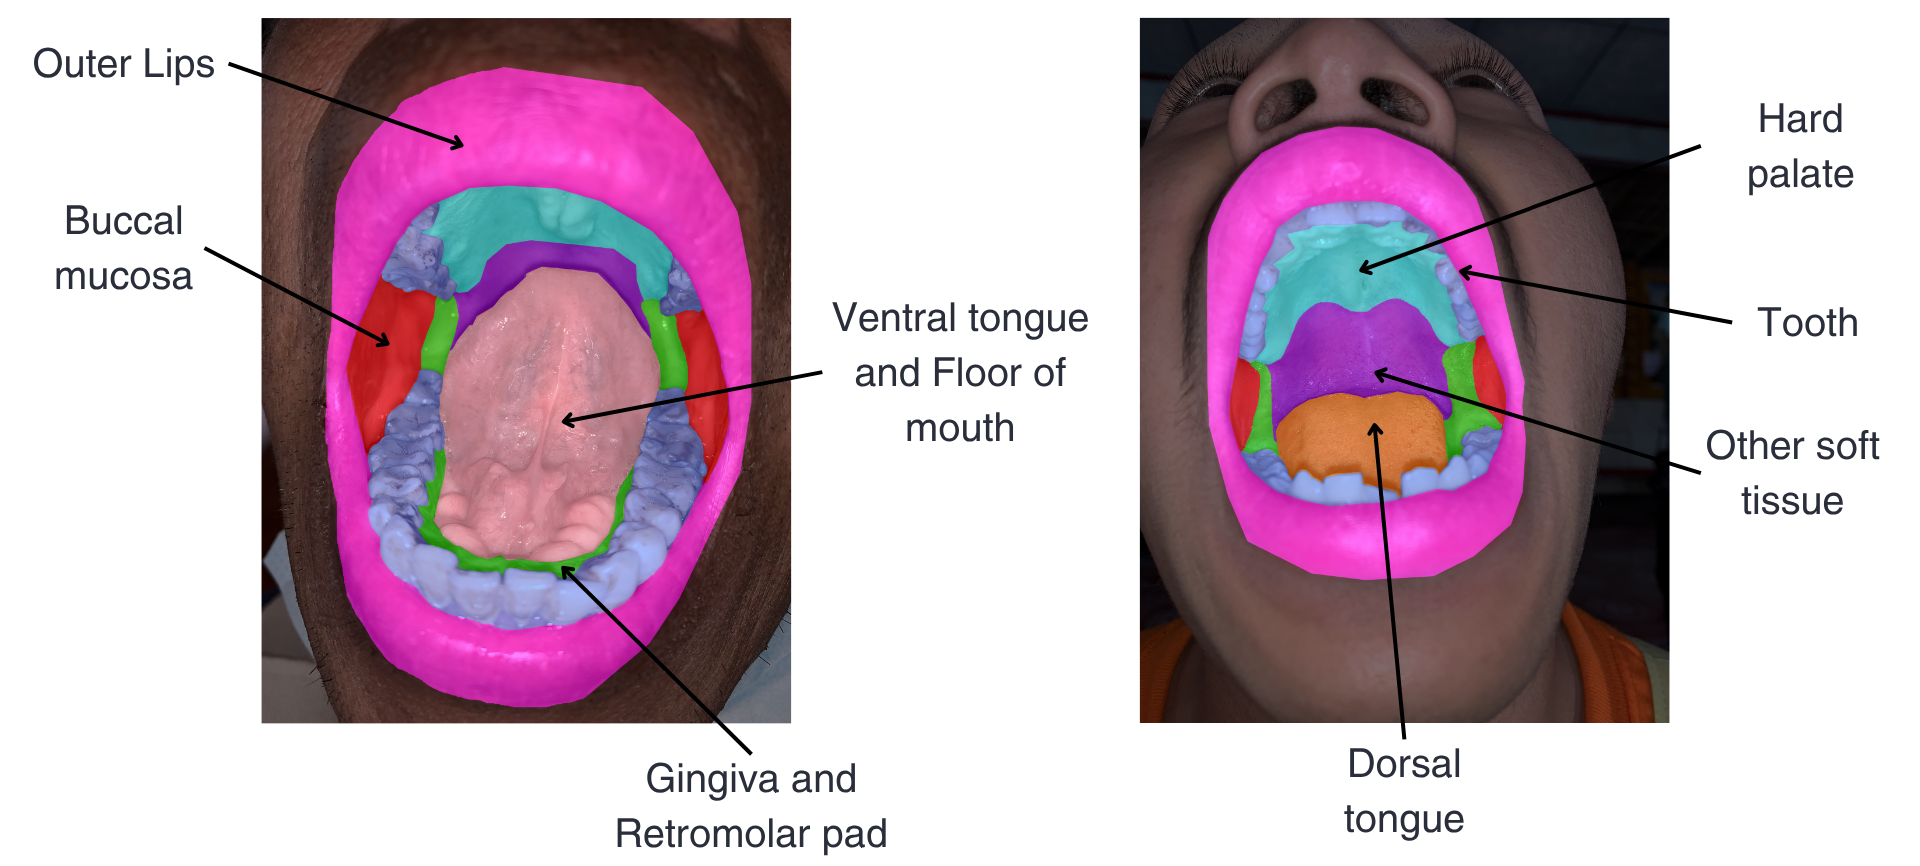
\includegraphics[width=0.9\linewidth]{images/ground_truth.png}
\end{center}
\caption[Poem]{ตัวอย่างภาพถ่ายช่องปากพร้อมผลเฉลย Ground truth ที่แสดงขอบเขตรอยโรค}
\label{fig:ground_truth}
\end{figure}


\section{การประมวลผลข้อมูลขั้นต้น (Preprocessing)}

ในขั้นตอนการเตรียมข้อมูล มีวัตถุประสงค์เพื่อปรับปรุงคุณภาพของข้อมูลก่อนนำเข้าสู่แบบจำลอง โดยเน้นการลดสัญญาณรบกวน และปรับโครงสร้างของวัตถุให้มีความสอดคล้องกับลักษณะทางกายวิภาค ซึ่งประกอบด้วยขั้นตอนดังต่อไปนี้

\subsection{การวิเคราะห์การกระจายขนาดวัตถุ (Object Size Distribution Analysis)}

ในขั้นตอนแรก ได้ดำเนินการวิเคราะห์การเชื่อมต่อของพิกเซล (connectivity analysis) โดยใช้เทคนิค connected component labeling เพื่อแยกวัตถุแต่ละชิ้นใน Ground truth ออกจากกัน จากนั้นทำการคำนวณขนาดของแต่ละวัตถุ และวิเคราะห์การกระจายตัวของขนาดวัตถุ (object size distribution)
ผลลัพธ์จากขั้นตอนนี้ถูกนำมาใช้ในการกำหนดเกณฑ์สำหรับการจำแนกวัตถุขนาดเล็กและวัตถุหลัก ซึ่งมีความสำคัญต่อขั้นตอนการปรับปรุงข้อมูลในลำดับถัดไป

\subsection{การรวมวัตถุขนาดเล็ก (Context-aware Small Object Merging)}

ในขั้นตอนนี้ ได้ดำเนินการปรับปรุงวัตถุขนาดเล็กโดยใช้การวิเคราะห์การเชื่อมต่อร่วมกับบริบทของวัตถุโดยรอบ (context-aware merging) โดยพิจารณาทั้งขนาดของวัตถุและความสัมพันธ์กับวัตถุข้างเคียง
เริ่มต้นจากการระบุ connected components ของแต่ละคลาส (ยกเว้น background) จากนั้นคำนวณสัดส่วนของขนาดวัตถุเทียบกับพื้นที่ของอวัยวะทั้งหมด เพื่อจำแนกว่าวัตถุใดจัดเป็นวัตถุขนาดเล็ก
\begin{equation}
\text{Ratio} = \frac{\text{Area}_{comp}}{\sum P_{anatomy}} \times 100
\end{equation}
โดยที่ $\text{Area}_{comp}$ คือจำนวนพิกเซลของวัตถุที่พิจารณา และ $\sum P_{anatomy}$ คือจำนวนพิกเซลรวมของทุกวัตถุที่ผ่านการทำ Labeling (คลาสที่ไม่ใช่ background) ในภาพนั้น ๆ

สำหรับวัตถุขนาดเล็ก จะทำการวิเคราะห์วัตถุข้างเคียงโดยใช้การขยายขอบเขต (dilation) เพื่อหาบริเวณที่สัมผัสกัน (contact area) ระหว่างวัตถุ จากนั้นเลือกวัตถุเป้าหมายสำหรับการรวม โดยพิจารณาจากจำนวนพิกเซลที่สัมผัสกันมากที่สุด และในกรณีที่มีค่าการสัมผัสเท่ากัน จะใช้ขนาดของวัตถุเป็นตัวตัดสิน
ในกรณีที่วัตถุขนาดเล็กไม่มีวัตถุข้างเคียงที่เหมาะสม จะถูกแปลงเป็น background เพื่อลดสัญญาณรบกวนในข้อมูล

นอกจากนี้ ยังมีการกำหนดเงื่อนไขเฉพาะสำหรับบางคลาส ได้แก่ การยกเว้นการรวมบริเวณสำหรับคลาสฟัน (Tooth) และริมฝีปาก (Lips) ที่มีขนาดเกินกว่าเกณฑ์สัญญาณรบกวนขั้นต่ำ เพื่อรักษาความถูกต้องเชิงกายวิภาคของข้อมูล

\subsection{การปรับปรุงช่องว่างภายในวัตถุ (Hole Refinement)}

ในขั้นตอนนี้ ได้ดำเนินการปรับปรุงบริเวณช่องว่างภายในวัตถุ โดยแบ่งออกเป็น 2 กระบวนการย่อย ได้แก่ การรวมพื้นหลังตามบริบท และการเติมเต็มช่องว่างเชิงโครงสร้าง

\subsubsection{การรวมพื้นหลังที่อยู่ภายในวัตถุ (Background Hole Merging)}

ในขั้นตอนนี้ ได้ทำการตรวจสอบพิกเซลคลาสพื้นหลัง (background) ที่อยู่ภายในวัตถุ โดยใช้การวิเคราะห์ connected components เพื่อระบุว่าเป็นบริเวณที่เป็นช่องว่าง (holes) ซึ่งถูกล้อมรอบด้วยวัตถุคลาสอื่น
เมื่อรู้แล้วว่ามี background components ที่อยู่ภายในวัตถุ จะทำการวิเคราะห์คลาสของพิกเซลรอบข้าง component นั้นๆ และเลือกคลาสที่มีจำนวนพิกเซลมากที่สุดเป็นคลาสเป้าหมาย จากนั้นทำการรวม component ดังกล่าวเข้ากับคลาสนั้น

\subsubsection{การเติมเต็มช่องว่างเชิงโครงสร้าง (Morphological Hole Filling)}

หลังจากรวมพื้นหลังที่อยู่ภายในวัตถุแล้ว ก็จะทำการเติมเต็มช่องว่างขนาดเล็กที่ยังคงหลงเหลืออยู่ โดยใช้เทคนิคทางสัณฐานวิทยา (morphological operations) เช่น การปิด (closing) ซึ่งเป็นการดำเนินการ dilation ตามด้วย erosion เพื่อเติมเต็มช่องว่างเล็กๆ ภายในวัตถุที่อาจเกิดจากความผิดพลาดในการทำ labeling หรือจากการรวมวัตถุขนาดเล็กในขั้นตอนก่อนหน้า
กระบวนการนี้ช่วยให้โครงสร้างของวัตถุมีความต่อเนื่องและสมบูรณ์มากยิ่งขึ้น

\section{การปรับปรุงผลลัพธ์ (Post-processing)}

หลังจากที่แบบจำลองทำการทำนายผลลัพธ์การแบ่งส่วนภาพแล้ว ได้มีการดำเนินการ post-processing เพื่อปรับปรุงความถูกต้องของผลลัพธ์ โดยเน้นการแก้ไขข้อผิดพลาดที่เกิดขึ้นจากการทำนายของโมเดล และปรับโครงสร้างของ segmentation mask ให้มีความสอดคล้องกับลักษณะทางกายวิภาคมากยิ่งขึ้น ซึ่งประกอบด้วยขั้นตอนดังต่อไปนี้

\subsection{การลบวัตถุขนาดเล็กและการเติมเต็มช่องว่าง (Small Object Removal and Hole Filling)}

ในขั้นตอนนี้ ได้ดำเนินการปรับปรุงผลลัพธ์เบื้องต้นโดยใช้แนวคิดเดียวกับ preprocessing ได้แก่ การลบ connected components ที่มีขนาดเล็กเกินไป ซึ่งมักเกิดจากการทำนายผิดพลาดของโมเดล (false positives) และการเติมเต็มช่องว่างภายในวัตถุ (hole filling) เพื่อให้โครงสร้างของ segmentation mask มีความสมบูรณ์มากยิ่งขึ้น
กระบวนการนี้ช่วยลดสัญญาณรบกวนและปรับปรุงความต่อเนื่องของวัตถุในภาพ

\subsection{การวิเคราะห์ความสัมพันธ์ระหว่างคลาส (Class Containment Analysis)}

จากการสังเกตผลลัพธ์ของแบบจำลองด้วยสายตา พบว่ามีข้อผิดพลาดในลักษณะที่คลาสหนึ่งครอบทับหรืออยู่ภายในอีกคลาสหนึ่ง (class containment) ในหลายกรณี ซึ่งส่งผลให้โครงสร้างของอวัยวะไม่สอดคล้องกับความเป็นจริง

ดังนั้น จึงได้พัฒนาเครื่องมือในการวิเคราะห์ความสัมพันธ์ระหว่างคลาส โดยใช้การวิเคราะห์การเชื่อมต่อของพิกเซล (connectivity analysis) ร่วมกับเทคนิค connected component labeling เพื่อระบุว่ามีวัตถุของคลาสใดที่ถูกล้อมรอบหรือครอบทับโดยวัตถุของอีกคลาสหนึ่ง
การวิเคราะห์ดังกล่าวช่วยให้สามารถระบุรูปแบบของข้อผิดพลาดที่เกิดขึ้นบ่อยในผลลัพธ์ของโมเดลได้อย่างเป็นระบบ

\subsection{การปรับปรุงผลลัพธ์ด้วยกฎเชิงตรรกะ (Rule-based Correction)}

จากผลการวิเคราะห์ความสัมพันธ์ระหว่างคลาส ได้นำข้อมูลที่ได้มาใช้ในการออกแบบกฎ (rule-based) สำหรับการปรับปรุงผลลัพธ์ โดยกำหนดเงื่อนไขในการแก้ไข label ของพิกเซลในบริเวณที่เกิด class containment
กฎดังกล่าวถูกออกแบบโดยอิงจากรูปแบบข้อผิดพลาดที่พบจริงในผลลัพธ์ของโมเดล เช่น การกำหนดว่าหากคลาสหนึ่งปรากฏอยู่ภายในอีกคลาสหนึ่งในลักษณะที่ไม่สอดคล้องกับโครงสร้างทางกายวิภาค จะทำการปรับ label ให้เหมาะสม
กระบวนการนี้ช่วยแก้ไขข้อผิดพลาดเชิงโครงสร้างที่โมเดลไม่สามารถเรียนรู้ได้โดยตรง และเพิ่มความสอดคล้องของผลลัพธ์กับลักษณะจริงของข้อมูล